\documentclass[tikz,border=10pt]{standalone}
% Scale s = 0.008484 cm/px (longest side 8 cm); origin at ink-bbox centre (546,449) px
\begin{document}
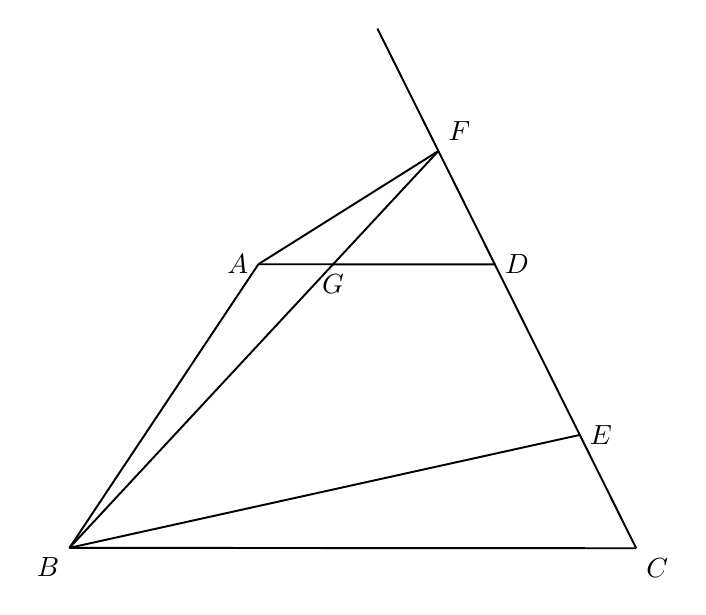
\begin{tikzpicture}[line width=0.7pt, line join=round,
  lbl/.style={font=\fontsize{10}{12}\selectfont}]

  % Named points (converted from pixel coordinates, y flipped)
  \coordinate (A) at (-1.2004919115161217,0.3487617408392347);
  \coordinate (B) at (-3.599466428046201,-3.2532033715437);
  \coordinate (C) at (3.598414154317942,-3.2583176333192645);
  \coordinate (D) at (1.80308321356366,0.3466276307666295);
  \coordinate (E) at (2.8816576233176616,-1.8191021643057805);
  \coordinate (F) at (1.086051668152344,1.786395316575422);
  \coordinate (G) at (-0.251201335771265,0.3480872477784118);
  \coordinate (T) at (0.3119530159819795,3.3407512332090468);   % far end of the long line (genuine overhang above F)

  % Base segment B-C
  \draw (B) -- (C);

  % Horizontal segment A-D (G lies on it)
  \draw (A) -- (D);

  % Segment F-B (passes through G)
  \draw (F) -- (B);

  % Segment F-A
  \draw (F) -- (A);

  % Segment A-B (missing edge restored from CV line_05)
  \draw (A) -- (B);

  % Long line through C, E, F, extending above F to T
  \draw (T) -- (C);

  % Segment E-B
  \draw (E) -- (B);

  % Point labels, offset outward
  \node[lbl, left] at (A) {$A$};
  \node[lbl, below left] at (B) {$B$};
  \node[lbl, below right] at (C) {$C$};
  \node[lbl, right] at (D) {$D$};
  \node[lbl, right] at (E) {$E$};
  \node[lbl, above right] at (F) {$F$};
  \node[lbl, below] at (G) {$G$};

\end{tikzpicture}
\end{document}
% GEOAGENT_REPAIR_V1 c18a466396f54661 363690ba43d89a1d77df1add2590b8c00f0853a08bf675435327dec07893dbc0
